\section{Results and Findings}
    

    \begin{frame}{Correlation Anlysis}
        \begin{columns}
        \begin{column}{0.5\textwidth}
        \begin{itemize}
            \item<1-> The figure illustrates the rolling 30-day correlation between differnt asset class.
            \item<2-> Bitcoin shows a moderate positive correlation with the S\&P 500 Index, while its relationships with COMEX Gold Futures and Aggregate Oil Futures are weaker and more variable, reflecting differing macroeconomic influences and market-specific dynamics.
           
        \end{itemize}
        \end{column}
        \begin{column}{0.6\textwidth}  %%<--- here
            \begin{center}
             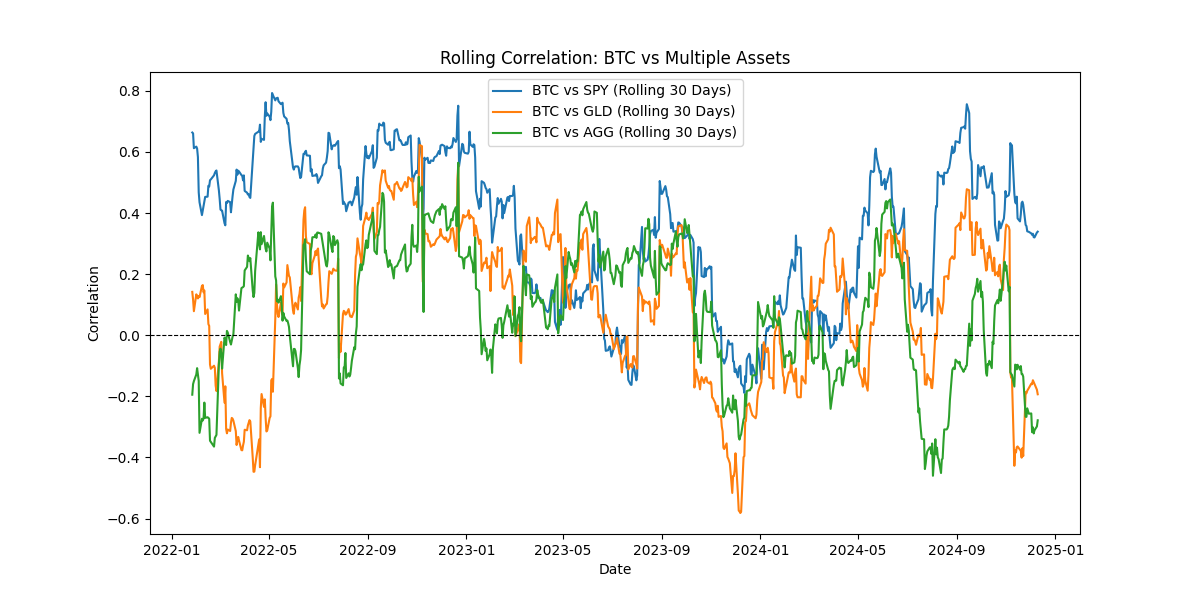
\includegraphics[width=\textwidth]{../../figure/rolling_correlation_multi.png}
             \end{center}
        \end{column}
        \end{columns}
    \end{frame}

    \begin{frame}{Vector Autoregression Model}
        \begin{columns}
        \begin{column}{0.5\textwidth}
        \begin{itemize}
            \item<1->Indicate no significant causal relationship between BTC and the selected traditional assets at the 5\% significance level. For AGG, GLD, and SPY, the p-values (0.977, 0.423, and 0.091, respectively) are above the critical threshold of 0.05
            
        \end{itemize}
        \end{column}
        \begin{column}{0.5\textwidth}  %%<--- here
            \begin{center}
             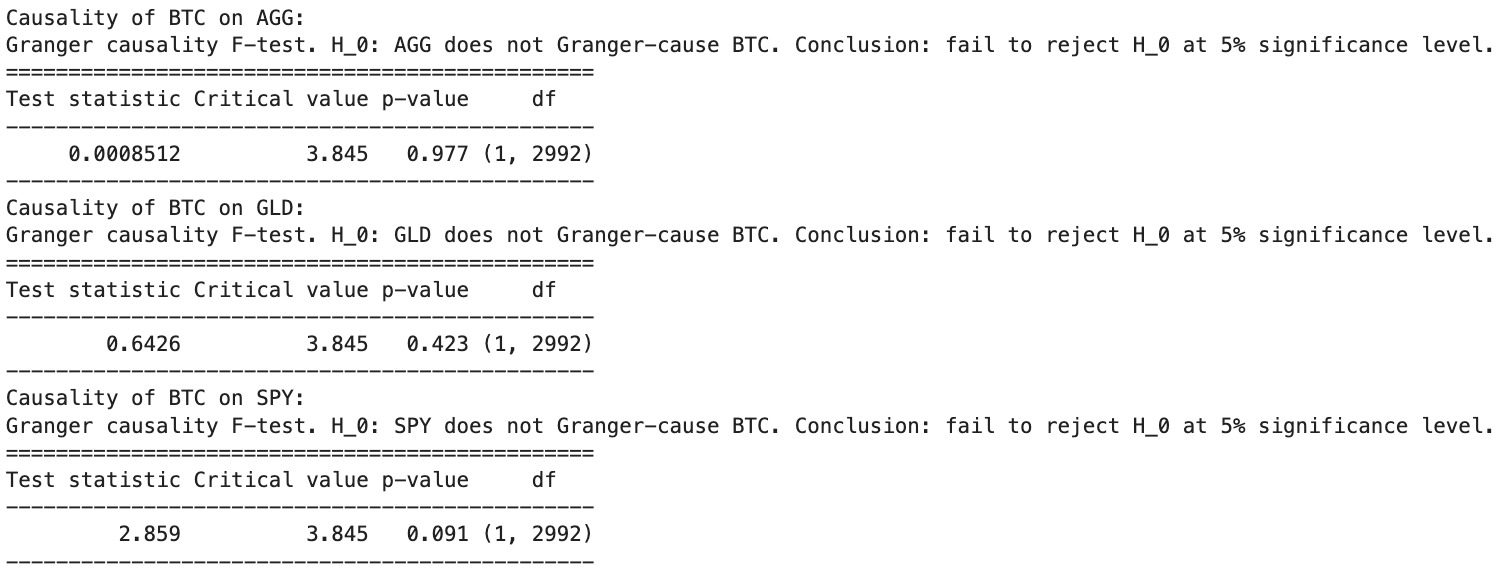
\includegraphics[width=\textwidth]{../../figure/var.png}
             \end{center}
        \end{column}
        \end{columns}
    \end{frame}
    \begin{frame}{Long Short-Term Memory Model}
        \begin{columns}
        \begin{column}{0.5\textwidth}
        \begin{itemize}
            \item<1-> The figure represents the heatmap of LSTM correlation matrix, revealing the relationships between the four financial assets.
            \item<2-> The matrix demonstrates an exceptionally high degree of correlation across all tradional assets
            \item<3-> But! Not bitcoin.In contrast to the earlier Pearson correlation analysis, which may have shown higher correlations in certain short-term market conditions, the LSTM heatmap reflects Bitcoin’s longer-term independence from traditional assets
        \end{itemize}
        \end{column}
        \begin{column}{0.5\textwidth}  %%<--- here
            \begin{center}
             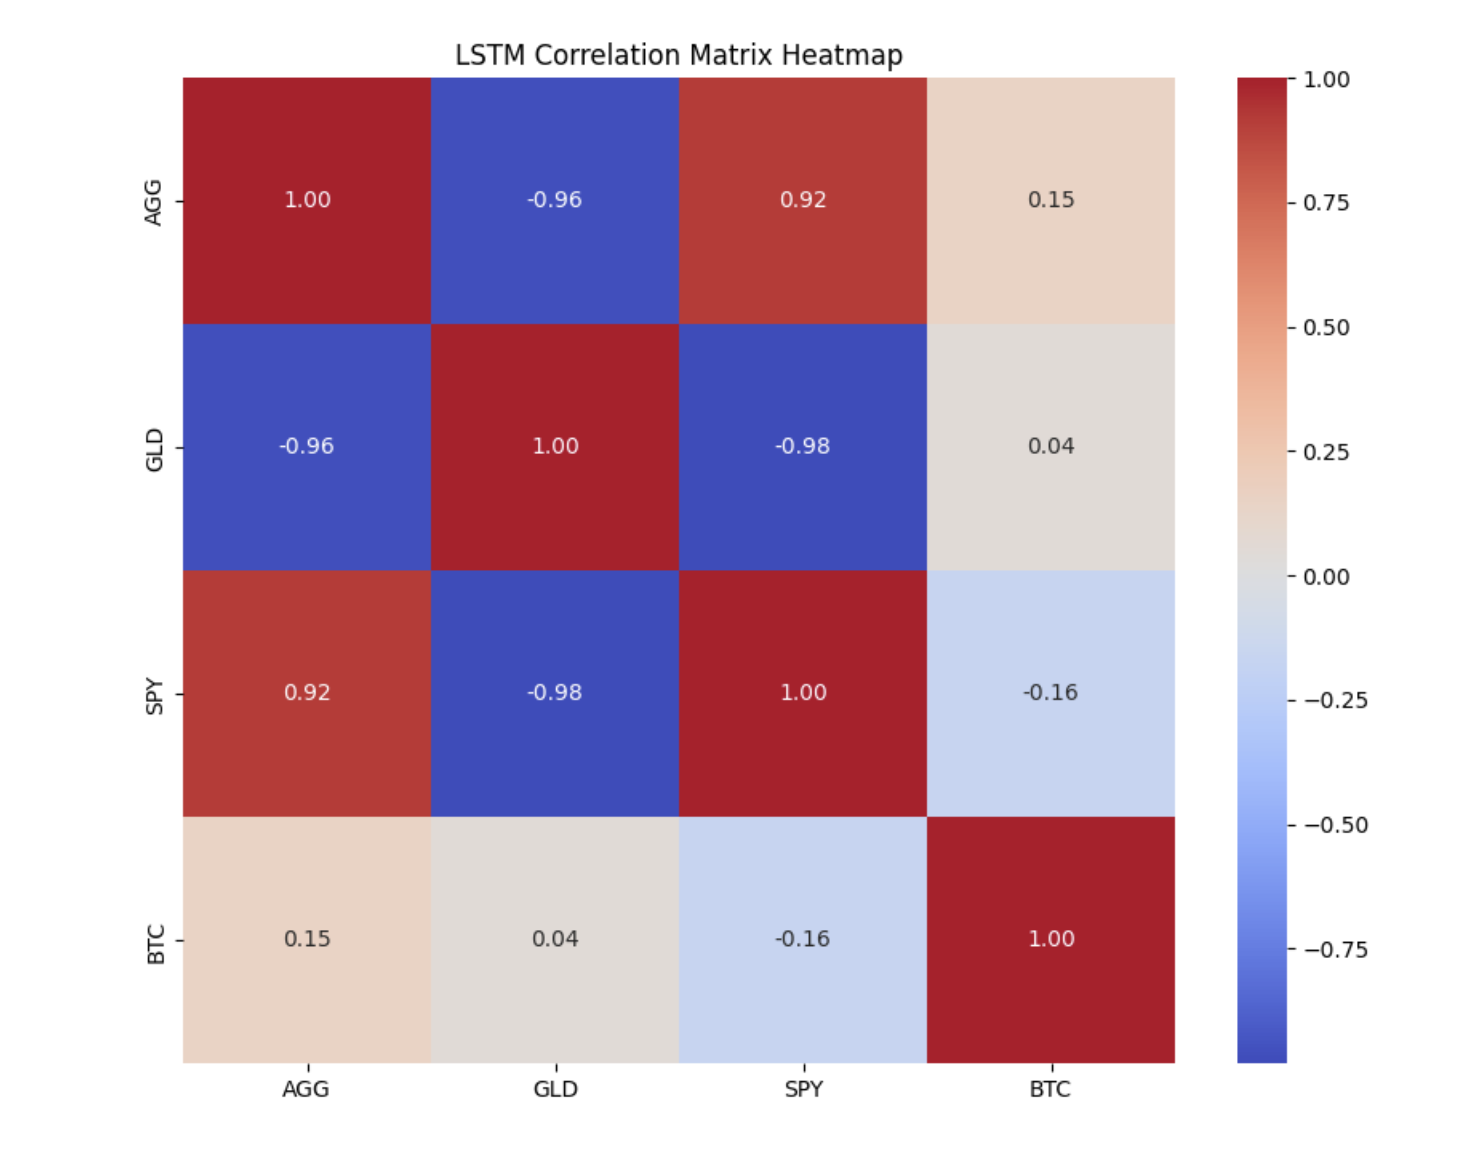
\includegraphics[width=\textwidth]{../../figure/lstm_correlation_heatmap_with_labels.png}
              \end{center}
        \end{column}
        \end{columns}
    \end{frame}


  
    
    